\documentclass[en,t]{sdqbeamer}
%\documentclass[c]{sdqbeamer}

\usepackage{listings}
\usepackage{graphicx}
\usepackage{tabularx}
\usepackage{multirow}
\usepackage{multicol}
\usepackage{tabulary}
\usepackage{colortbl}
\usepackage{tikzsymbols}
\usepackage{tikz}
\usepackage{booktabs}
\usetikzlibrary{positioning,fit,shapes}
\usepackage[lined,linesnumbered,ruled,noend]{algorithm2e}
\usepackage{bm}
\usepackage{forloop}

\hypersetup{
	colorlinks=true,
	urlcolor=kit-orange
}

% set sdqbeamer options
\titleimage{blender-render}
\groupname{Algorithm Engineering}
\grouplogo{ae}
%\selectlanguage{english}


\usepackage[backend=biber,style=numeric-comp,sorting=none]{biblatex}
\addbibresource{references.bib}

% define title etc.pp.
\title[SAT Solving]{Practical SAT Solving}
\subtitle{Lecture 13: Proofs: Pragmatics \& Parallel Production}
\author{{Markus Iser}, \underline{Dominik Schreiber}, Tom\'a\v{s} Balyo}
\date{July 15, 2024}

% Existing KIT colors: kit-green, kit-blue, kit-red, kit-gray, kit-orange, kit-lightgreen, kit-brown, kit-purple, kit-cyan
% configure appearance
\setbeamercolor{block title}{bg=kit-blue}
\setbeamercolor{block body}{bg=kit-blue!10}
\setbeamercolor{block title example}{bg=kit-orange}
\setbeamercolor{block body example}{bg=kit-orange!10}
\setbeamertemplate{itemize item}{\color{kit-gray}\textbullet}
\setbeamertemplate{itemize subitem}{\color{kit-gray}\textbullet}
\setbeamercolor{item projected}{bg=kit-gray, fg=kit-gray}
\renewcommand{\insertnavigation}[1]{} % remove navigation bar

% define commands
\definecolor{myblue}{HTML}{0D3B66}
\definecolor{myred}{HTML}{6E0E0A}
\definecolor{mypink}{HTML}{F7B2B7}

\newcommand{\vars}[1]{\textsf{vars} (#1)}
\newcommand{\lits}[1]{\textsf{lits} (#1)}
\newcommand{\clss}[1]{\textsf{clss} (#1)}

\newcommand{\highl}[1]{\textcolor{myblue}{#1}}
\newcommand{\highlo}[1]{\textcolor{myred}{#1}}
\newcommand{\highlow}[1]{\textcolor{mypink}{#1}}

% Extra column types for tabularx
\newcolumntype{C}{>{\centering\arraybackslash}X}
\newcolumntype{L}{>{\raggedright\arraybackslash}X}
\newcolumntype{R}{>{\raggedleft\arraybackslash}X}

\newcommand{\setcolsep}[1]{\setlength{\tabcolsep}{#1}}
\newcommand{\setrowsep}[1]{\renewcommand{\arraystretch}{#1}}

% Definitions for the Tseitin transformation
\newcommand{\true}{\ensuremath{\mathit{True}}}
\newcommand{\false}{\ensuremath{\mathit{False}}}
\newcommand{\allvars}{\ensuremath{\mathcal{V}}}
\newcommand{\tseitin}[1]{\ensuremath{\mathcal{T}(#1)}}
\newcommand{\tseitinRec}[2]{\ensuremath{\mathcal{T}^{#2}(#1)}}
\newcommand{\tseitinSym}[1]{\ensuremath{\mathcal{T}_\mathsf{lit}(#1)}}
\newcommand{\tseitinDef}[2]{\ensuremath{\mathcal{T}_\mathsf{def}^{#2}(#1)}}
\newcommand{\hcancel}[2][black]{\setbox0=\hbox{$#2$}\rlap{\raisebox{.45\ht0}{\textcolor{#1}{\rule{\wd0}{1pt}}}}#2} 
\newcommand{\sateq}{\mathrel{\overset{\makebox[0pt]{\mbox{\normalfont\tiny\sffamily SAT}}}{=}}}

\newcommand{\enc}{\ensuremath{\mathcal{E}}} % encoding

% exercise commands
\newcommand{\exhead}[3]{
\hrule~\\[1ex]\noindent
{\bf Practical SAT Solving} (ST 2024) \hfill \fbox{Assignment #1} \\[1ex]
Markus Iser, Dominik Schreiber, Tom\'a\v{s} Balyo\\[1ex]
Algorithm Engineering (KIT) \hfill #2 -- #3\\
\hrule
\thispagestyle{empty}
}


\renewcommand{\highl}[1]{\textcolor{kit-blue}{#1}}
\renewcommand{\highlo}[1]{\textcolor{kit-orange}{#1}}
\newcommand{\unimp}[1]{\textcolor{gray}{#1}}

% Redefine `\rowcolor` to allow a beamer overlay specifier
% New syntax: \rewcolor<overlay>[color model]{color}[left overhang][right overhang]
\makeatletter
% Open `\noalign` and check for overlay specification:
\def\rowcolor{\noalign{\ifnum0=`}\fi\bmr@rowcolor}
\newcommand<>{\bmr@rowcolor}{%
    \alt#1%
        {\global\let\CT@do@color\CT@@do@color\@ifnextchar[\CT@rowa\CT@rowb}% Rest of original `\rowcolor`
        {\ifnum0=`{\fi}\@gooble@rowcolor}% End `\noalign` and gobble all arguments of `\rowcolor`.
}
% Gobble all normal arguments of `\rowcolor`:
\newcommand{\@gooble@rowcolor}[2][]{\@gooble@rowcolor@}
\newcommand{\@gooble@rowcolor@}[1][]{\@gooble@rowcolor@@}
\newcommand{\@gooble@rowcolor@@}[1][]{\ignorespaces}
\makeatother

% Redefine '\cellcolor' for beamer overlay use
\renewcommand<>\cellcolor[1]{\only#2{\beameroriginal\cellcolor{#1}}}

\begin{document}

\begin{frame}
	\thispagestyle{empty}
	\titlepage
\end{frame}

% \begin{minipage}[c][8cm][t]{0.65\textwidth}

\begin{frame}{Overview}
	\textbf{Last lectures}
	\begin{itemize}
		\item Background on \highl{proof systems}, proof complexity
		\item Connections to \highl{preprocessing}
	\end{itemize}
	
	\vspace*{3mm}
	\textbf{This lecture}
	\begin{itemize}
		\item Common state-of-the-art \highl{proof formats}
		\item Pragmatics of \highl{proof production} and \highl{checking}
		\item Producing proofs with \highl{parallel + distributed solvers}
		\item Beyond proof files: \highl{on-the-fly checking}
	\end{itemize}
\end{frame}

\begin{frame}{Back To Basics}
	\begin{itemize}
		\item Solver on unsat.\ formula $F$ produces \highl{sequence of clauses} $P := \langle c_1, c_2, \ldots, c_n \rangle$ with $c_n = \emptyset$
		\item Goal: \highl{Justify} for $i=1, \ldots, n$ that $F \models c_{i}$, i.e., that $c_i$ follows from $F$\\[1mm]
		-- actually (in practice): that (\,\highl{$F \cup \bigcup_{j=1}^{i-1} c_{j}$}\,) $\models c_i$
		\item \textbf{Clausal Proof} $\mathcal{P}$: Expression of $P$ with \highl{all information needed} to justify all steps \pause \highlo{efficiently (?)}
	\end{itemize}

	\vspace*{3mm}
	\pause
	\begin{block}{Approach 1: Basic Clausal Proof}
		\begin{itemize}
			\item \textbf{Solving}: Solver just \highl{logs each produced $c_i$} to a file\ \ \ $\Rightarrow$\ \ $\mathcal{P} = P$
			\item \textbf{Checking}: Maintain clause database $B$ initialized as $B := F$;\\
			for each $c_i$, \highl{confirm that $B \models c_i$} and then \highl{$B := B \cup c_i$}
			\pause
			\item \highlo{How do we perform the confirmation step?}
	\end{itemize}
	\end{block}
\end{frame}

\begin{frame}{Efficient Redundancy Checking~\cite{van2008verifying}}
	
	\vspace*{-2mm}
	\begin{block}{The RUP Property}
		Given a clause set $C$ and a clause $c$, we say that $c$ has the \highl{Reverse Unit Propagation} (RUP) property iff\\
		unit propagation on $(C \cup \{\overline{c}\})$, where $\overline{c} := \{ \neg l\ :\ l \in c \}$, produces the \highlo{empty clause}.
	\end{block}
	\begin{itemize}
		\item Is a clause $c$ with RUP property w.r.t.\ a checker's clause set $B$ a sound addition to $B$?\\
		-- \highl{Yes}:\ \ \ $B \wedge \bigwedge_{l \in c} \neg l$ is unsatisfiable\ \ \ $\rightarrow$\ \ \ No way to satisfy $B$ without satisfying $c$\ \ \ $\rightarrow$\ \ \ $B \models c$
		\pause
		\item What kinds of clauses \highl{have} the RUP property?
		\begin{itemize}
			\item Conflict clauses from CDCL
			\item Clauses arising from many pre-- and inprocessing techniques\\
			(variable elimination, subsumption, vivification, \ldots)
			\item Actually, \highl{all clauses} produced by out-of-the-box \textsc{CaDiCaL}
		\end{itemize}
		\pause
		\item What kinds of clauses \highlo{do not have} the RUP property?
		\begin{itemize}
			\item \highl{Extended Resolution} steps
			\item Propagation Redundancy (PR) clauses
			\item \ldots
		\end{itemize}
	\end{itemize}
\end{frame}

\begin{frame}{RUP Proof Checking}
	
	\vspace*{-3mm}
	\begin{block}{Approach 2: RUP Proof}
			\textbf{Solving}: Solver just \highl{logs each produced $c_i$} to a file\ \ \ $\Rightarrow$\ \ $\mathcal{P} = P$.\\
			
			\textbf{Checking}:\\[2mm]
			\hspace*{0.5cm}\begin{minipage}{10cm}
				$B := F$\\
				\textbf{for} $i=1,\ldots,n$:\\
				\hspace*{1cm} propagate $\neg l$ in $B$ for each $l \in c_i$ \\
				\hspace*{1cm} \textbf{if} propagation in $B$ does \textit{not} yield the empty clause: \\
				\hspace*{2cm} \textbf{return} \textbf{\highlo{ERROR}} \\
				\hspace*{1cm} undo propagations in $B$ \\
				\hspace*{1cm} \highl{$B := B \cup c_i$} \\
				\textbf{return} \textbf{\highl{VALIDATED}}
			\end{minipage}
	\end{block}

	\pause
	\vspace*{2mm}
	\textbf{Checking complexity:} \pause $\mathcal{O}(|B|)$ per step $\Rightarrow$ \highlo{$\mathcal{O}(|P|^2)$} for $|P| \gg |F|$ \\
	\textbf{Checking space usage:} \pause \highlo{$\mathcal{O}(|F| + |P|)$}
	\hfill How to improve on \highl{both}?
\end{frame}

\begin{frame}{From RUP to DRUP~\cite{heule2013trimming}}
	Actually, a solver also \highl{deletes} clauses. $\Rightarrow$ \highl{Put deletion information in the proof!}
	\begin{itemize}
		\item $\mathcal{P} = (o_1, \ldots, o_N)$ where $o_i = (op_i, c_i)$\\
		-- $op_i \in \{\texttt{add}, \texttt{delete}\}$\\
		-- \texttt{delete}:\ \ $c_i$ is a clause added by some $o_j$, $j<i$, and \highlo{not \texttt{delete}d} by any $o_k$, $j<k<i$\\
		-- \highl{multi-set semantics} possible where a clause may be added (+ deleted) multiple times
	\end{itemize}

	\pause
	\vspace*{3mm}
	\begin{center}
		\begin{minipage}[c][8cm][t]{0.4\textwidth}
			\textbf{Formula:}\\[1mm]
			\ttfamily\small
			$\phantom{\wedge \ }x_1 \vee \neg x_2$ \\
			$\wedge \ x_2 \vee \neg x_4$ \\
			$\wedge \ x_1 \vee x_2 \vee x_4$ \\
			$\wedge \ \neg x_1 \vee \neg x_3$ \\
			$\wedge \ x_1 \vee \neg x_3$ \\
			$\wedge \ \neg x_1 \vee x_3$ \\
			$\wedge \ x_1 \vee x_3 \vee \neg x_4$ \\
			$\wedge \ x_1 \vee x_3 \vee x_4$
		\end{minipage}%
		\begin{minipage}[c][8cm][t]{0.4\textwidth}
			\textbf{Proof:}\\[1mm]
			\ttfamily\small
			\highl{add} $\neg x_3$\\
			\highl{add} $x_1 \vee x_2$\\
			\highl{add} $\neg x_1$\\
			\highlo{del} $\neg x_3$\\
			\highl{add} $x_2 \vee x_3 \vee \neg x_4$\\
			\highl{add} $x_1 \vee x_2 \vee x_3$\\
			\highl{add} $\emptyset$
		\end{minipage}
	\end{center}
\end{frame}

\begin{frame}{DRUP}
	\begin{block}{Approach 3: DRUP (Deletion RUP) Proof}
		\hspace*{0.5cm}\begin{minipage}{10cm}
			$B := F$\\
			\textbf{for} $i=1,\ldots,$\highl{$N$}:\\
			\hspace*{1cm} \highl{\textbf{if} $op_i =$ \texttt{delete}:} \\
			\hspace*{2cm} \highl{$B := B \setminus c_i$} \\
			\hspace*{2cm} \highl{\textbf{continue}} \\
			\hspace*{1cm} propagate $\neg l$ in $B$ for each $l \in c_i$ \\
			\hspace*{1cm} \ldots\ \ \ \textcolor{gray}{// continue as in RUP Proof}
		\end{minipage}
	\end{block}

	\vspace*{2mm}
	\textbf{Correctness:} \pause deleting clauses only makes a clause set \highl{more satisfiable} $\checkmark$\\
	\textbf{Complexity:} \pause \highl{$\mathcal{O}(|P| \times M)$} where $M$ is the \highl{max.\ volume of present clauses} during solving \\
	\textbf{Space usage:} \pause \highl{$\mathcal{O}(M)$} \ \ \ \ $\Rightarrow$ ``\highl{fits into RAM if solving fits into RAM}''

	\vspace*{2mm}
	Can we further improve running time?
\end{frame}

\begin{frame}{From DRUP to LRUP~\cite{cruz2017efficient}}
	
	\vspace*{-2mm}
	\textbf{Idea:} Enrich proof to \highl{accelerate unit propagation} (UP) of $\overline{c_i}$ through $B$
%	\textbf{Improvement:} Let solver output \highl{``hints'' to accelerate UP}!
	\begin{itemize}
		\item $\mathcal{P} = (o_1, \ldots, o_N)$ where $o_i = (\texttt{add}, id_i, c_i, d_i)$ \textbf{or} $o_i = (\texttt{delete}, id_i)$\\
		-- $id_i \in \mathbb{N}^+$,\ \ $d_i = \langle d_{i1}, \ldots, d_{ik_i} \rangle$ where $d_{ij} \in \mathbb{N}^+$, $k_i \in \mathbb{N}^+$\\
		%-- $c_i$ and $d_i$ are unused if $op_i = \textit{delete}$
		%\item Each clause has an \highl{ID}: 1, \ldots, $|V|$ for original clauses, $|V|+1, \ldots$ for derived clauses
		\item With $d_i$, solver references earlier clauses which \highl{UP needs to look at} to arrive at the empty clause\\
		-- for $1 \leq j < k_i$, clause \highl{\#\,$d_{ij}$} (i.e., the clause referred to by $d_{ij}$) must \highl{break down into a unit}\\
		-- clause \#\,$d_{ik_i}$ must \highl{break down into $\emptyset$}
	\end{itemize}

	\pause
	\vspace*{3mm}
	\begin{center}
	\begin{minipage}[c][8cm][t]{0.3\textwidth}
		\textbf{Formula:}\\[1mm]
		\ttfamily\small
		(1) $x_1 \vee \neg x_2$ \\
		(2) $x_2 \vee \neg x_4$ \\
		(3) $x_1 \vee x_2 \vee x_4$ \\
		(4) $\neg x_1 \vee \neg x_3$ \\
		(5) $x_1 \vee \neg x_3$ \\
		(6) $\neg x_1 \vee x_3$ \\
		(7) $x_1 \vee x_3 \vee \neg x_4$ \\
		(8) $x_1 \vee x_3 \vee x_4$
	\end{minipage}%
	\begin{minipage}[c][8cm][t]{0.3\textwidth}
		\textbf{DRUP Proof:}\\[1mm]
		\ttfamily\small
		\highl{add} $\neg x_3$\\
		\highl{add} $x_1 \vee x_2$\\
		\highl{add} $\neg x_1$\\
		\highlo{del} $\neg x_3$\\
		\highl{add} $x_2 \vee x_3 \vee \neg x_4$\\
		\highl{add} $x_1 \vee x_2 \vee x_3$\\
		\highl{add} $\emptyset$
	\end{minipage}%
	\begin{minipage}[c][8cm][t]{0.3\textwidth}
		\textbf{LRUP Proof:}\\[1mm]
		\ttfamily\small
		\highl{add} (9) $\neg x_3$ \ \ (5, 4)\\
		\highl{add} (10) $x_1 \vee x_2$ \ \ (3, 2)\\
		\highl{add} (11) $\neg x_1$ \ \ (6, 9)\\
		\highlo{del} (9) \\
		\highl{add} (12) $x_2 \vee x_3 \vee \neg x_4$ \ \ (7, 11)\\
		\highl{add} (13) $x_1 \vee x_2 \vee x_3$ \ \ (8, 12)\\
		\highl{add} (14) $\emptyset$ \ \ (11, 10, 1)\\
	\end{minipage}
	\end{center}
\end{frame}

\begin{frame}{LRUP}
	\vspace*{-3mm}
	\begin{block}{Approach 4: LRUP (Linear RUP) Proof Checking}
		\hspace*{0.5cm}\begin{minipage}{14cm}
			$B := F$\\
			\textbf{for} $i=1,\ldots,N$:\\
			\hspace*{5mm} {\textbf{if} $op_i =$ \texttt{delete}:} \\
			\hspace*{10mm} {$B := B \setminus \{\#\,id_i\}$} \ \ \ \textcolor{gray}{// delete clause referred to by $id_i$} \\
			\hspace*{10mm} {\textbf{continue}} \\
			\hspace*{5mm} $U := \{ \overline{l}\ :\ l \in c_i \}$ \\
			\hspace*{5mm} \textbf{for} $j=1,\ldots,k-1$: \\
			\hspace*{10mm} \textbf{assert}: clause \#\,$d_{ij}$ under $U$ becomes a unit clause $\{u\}$ \ \ \ \textcolor{gray}{// returns \textbf{\highlo{ERROR}} upon failure} \\
			\hspace*{10mm} $U := U \cup \{u\}$ \\
			\hspace*{5mm} \textbf{assert}: clause \#\,$d_{ik_i}$ under $U$ becomes the empty clause \ \ \ \textcolor{gray}{// returns \textbf{\highlo{ERROR}} upon failure} \\
			\hspace*{5mm} $B := B \cup \{c_i\}$ \ \ \ \textcolor{gray}{// confirmed: $B \cup \{\overline{c_i}\} \models \emptyset$ } \\
			\textbf{return} \textbf{\highl{VALIDATED}}
		\end{minipage}
	\end{block}
	\vspace*{2mm}
	$\Rightarrow$ \highlo{Larger proofs} but \highl{much more efficient checking} (often $10\times$ or more)
\end{frame}

\begin{frame}{From (D|L)RUP to (D|L)RAT~\cite{heule2016drat}}
	\vspace*{-2mm}
	\begin{block}{Resolution Asymmetric Tautology \textcolor{gray!50}{(recap)}}
		Clause $c$ has the \emph{Resolution Asymmetric Tautology} (RAT) property in $F$ w.r.t.\ literal $x \in c$\\
		iff \highlo{every resolvent} $c' \in \{c \otimes_x \tilde{c}\ |\ \tilde{c} \in F_{\overline{x}} \}$ has the \highl{RUP property} in $F$.
	\end{block}
	\vspace*{1mm}
	\pause
	``Only'' requiring each clause $c_i \in P$ to have the \highl{RAT property} (rather than RUP) allows for \highl{stronger proofs}!
	\begin{itemize}
		\item For RAT clause $c$, $F \cup c$ is \highl{satisfiability-preserving} to $F$ but may be \highlo{not equivalent} to $F$
		\item Allows to express satisfiability-preserving transformations like \highl{variable addition}
		\item \highl{As powerful as Extended Resolution}
	\end{itemize}
	\vspace*{1mm}
	\pause
	How to incorporate RAT into proof checking?
	\vspace*{1mm}
	\begin{itemize}
		\item DRUP $\rightarrow$ \textbf{DRAT}: \ \ For each added clause $c_i$, find \highl{pivot literal $x \in c_i$} and confirm that $c_i$ is RAT in $B$ w.r.t.\ $x$
		\begin{itemize}
			\item Convention: \highl{1st literal of $c_i$} must be valid pivot
			\item Find all resolvents, check RUP for every one of them
		\end{itemize}
		\pause
		\vspace*{1mm}
		\item LRUP $\rightarrow$ \textbf{LRAT}: \ \ Additions $(\texttt{add}, id_i, c_i, d_i\highl{, r_i})$ with $r_i = \langle r_{i1}, \ldots, r_{im_i} \rangle$, $m_i \in \mathbb{N}_0$
		\begin{itemize}
			\item Each $r_{ij}$ references a clause $\tilde{c}$ and the required RUP steps for $c' = c_i \otimes_x \tilde{c}$\ \ \textcolor{gray}{(like $d_i$ for $c_i$ in pure RUP)}
			\item Still need to internally maintain \highl{occurrences of each literal} to check that all $\tilde{c}$ are covered
		\end{itemize}
	\end{itemize}
\end{frame}

\begin{frame}{Proof (File) Formats: DRAT and LRAT}
	
	\vspace*{0mm}
	\centering
	
\includegraphics[height=5.2cm]{figures/l13/proof-formats.pdf}\\[2mm]
	
	\unimp{These proofs only feature RUP additions. \ \ In an LRAT addition, each $r_{ij}$ is written as the negated ID of $\tilde{c}$\\
		followed by IDs for the RUP steps of $c'$.}
\end{frame}

\begin{frame}{Adding Proof Support to Solvers}
	
	\vspace*{-2mm}
	I wrote my own CDCL SAT solver. How can I let it \highl{produce UNSAT proofs}?
	\pause
	
	\vspace*{2mm}
	\textbf{DRAT:} \ \ \highl{super simple!}
	\begin{itemize}
		\item Create an (empty) proof file at upstart
		\item Log each new redundant clause {\small (including the empty clause)} into the proof file
		\item Log each discarded clause into the proof file, prepended with ``\texttt{d}''
		%\item For UNSAT, the final learned clause should be the empty clause
	\end{itemize}

	\pause
	\vspace*{2mm}
	\textbf{LRAT:} \ \ Clause addition lines need to be enriched \highlo{with dependency information (``hints'')}
	\begin{itemize}
		\item CDCL conflict clauses: \highl{simple} -- use conflict's \highl{implication graph}
		\item \highlo{Additional effort} for each employed pre-/inprocessing technique
	\end{itemize}

	\pause
	\vspace*{2mm}
	\textbf{Other formats:}
	\begin{itemize}
		\item \highl{FRAT}: Compromise between DRAT and FRAT at the developer's discretion \cite{baek2022flexible}
		\item \highl{DPR, LPR}: Propagation Redundancy (PR) reasoning \cite{balyo2023proceedings}
		\item \highl{VeriPB}: Pseudo-Boolean reasoning \cite{balyo2023proceedings}
	\end{itemize}

	\vspace*{2mm}
	{Note:} \highl{formally verified checkers} are available for \highl{all these formats} \unimp{(sometimes translation-based)}
\end{frame}

\begin{frame}{Proof Production: The Parallel Case}
	\textbf{What about proofs from parallel solvers?}
	\begin{itemize}
		\item Pure portfolios: \pause \highl{trivial} if each participant produces a proof
		\item Search space splitting solvers: \pause straight forward to \highl{stitch together proofs} for sub-problems (e.g., \cite{heule2016solving})
		\item Clause-sharing solvers: \pause \highlo{more difficult} due to \highlo{cross-references between solvers' clauses} \cite{heule2014validating}
	\end{itemize}

	\vspace*{2mm}
	\textbf{Before 2023:} \highlo{Large gap of trustworthiness} between best sequential and best parallel (clause-sharing) solvers\\[2mm]
	\pause
	\textbf{2023:} \highl{LRAT-based proofs from clause-sharing solvers} \cite{michaelson2023unsatisfiability}
	\begin{itemize}
		\item \highl{Globally unique clause IDs} without communication\\
		-- for $o$ original clauses and $p$ solver threads, the $i$-th thread assigns clause IDs \highl{$o + i + kp$} ($k \in \mathbb{N}_0$)
		\item After solving, \highl{rewind the procedure}, using ``hints'' of LRAT to \highl{trace dependencies of empty clause}
		\item Funnel all clauses marked as required into a \highl{single, ordered proof file}
	\end{itemize}
\end{frame}


\newcounter{animcount}
\begin{frame}{Distributed Proof Production (1/2) \ \ \cite{michaelson2023unsatisfiability}}%
	\hspace{0.73cm} --- Produced Clauses $\rightarrow$\\[0.2cm]
	\begin{minipage}{0.05\textwidth}%
		\noindent $S_1$\\[0.7cm]%
		\noindent $S_2$\\[0.7cm]%
		\noindent $S_3$\\[0.7cm]%
		\noindent $S_4$
	\end{minipage}%
	\begin{minipage}{0.95\textwidth}
		\forloop{animcount}{01}{\value{animcount} < 17}{%
			\def\imgname{figures/l13/depgraph/dependency-graph-\arabic{animcount}.png}\only<\value{animcount}>{\includegraphics[width=\textwidth]{\imgname}}%
		}
	\end{minipage}
	
	\vspace*{1mm}
	\hfill\unimp{\footnotesize Random 3-SAT formula, 180 variables.\ \ 4 notebook cores $\times$ 1.7\,s.\ \ 300k dependencies (w/o orig.\ clauses).}
	
	\vspace{0.35cm}
	\only<-8>{\textbf{Solving}: Each thread \highl{derives and shares} clauses, logs to \highl{partial proof file}} %\highl{Angleichen von Klausel-IDs} an jeder \highl{Klauselaustausch-Epoche}}%
\only<9->{\textbf{Reconstruction}: \highl{Trace} required clauses, \highl{revert} each clause exchange}%
\textcolor{white}{Gg}%
\end{frame}

\begin{frame}{Distributed Proof Production (2/2) \ \ \cite{michaelson2023unsatisfiability}}
	\begin{minipage}{0.4\textwidth}
		\textbf{Merging:}\\
		
		\hspace*{-4mm}
		\begin{minipage}{\textwidth}
			\begin{itemize}
				%\addtolength{\itemsep}{0.5\baselineskip}
				\item Funnel required clause additions, \highl{still in reverse order}, into singular proof file
				%\item $k$ input streams of sorted proof lines:\\
				%Consume \highl{highest ID first}\\
				%$\rightsquigarrow$ single sorted output stream
				\item \highl{Hierarchical merging} along tree
				\item ``Root process'' writes output to file\\[1mm]
				%\setbeamertemplate{enumerate items}[square]
				-- Seeing an ID $d_{ij}$ \highl{for the first time}?\\
				\phantom{-- }$\Rightarrow$ write \highl{deletion of $d_{ij}$} before writing\\
				\phantom{-- $\Rightarrow$ }the current statement!\\[1mm]
				-- Finally: \highl{Invert lines of proof file}
			\end{itemize}
		\end{minipage}
	\end{minipage}%
	\begin{minipage}{0.6\textwidth}
		\centering
		\vspace*{1mm}
		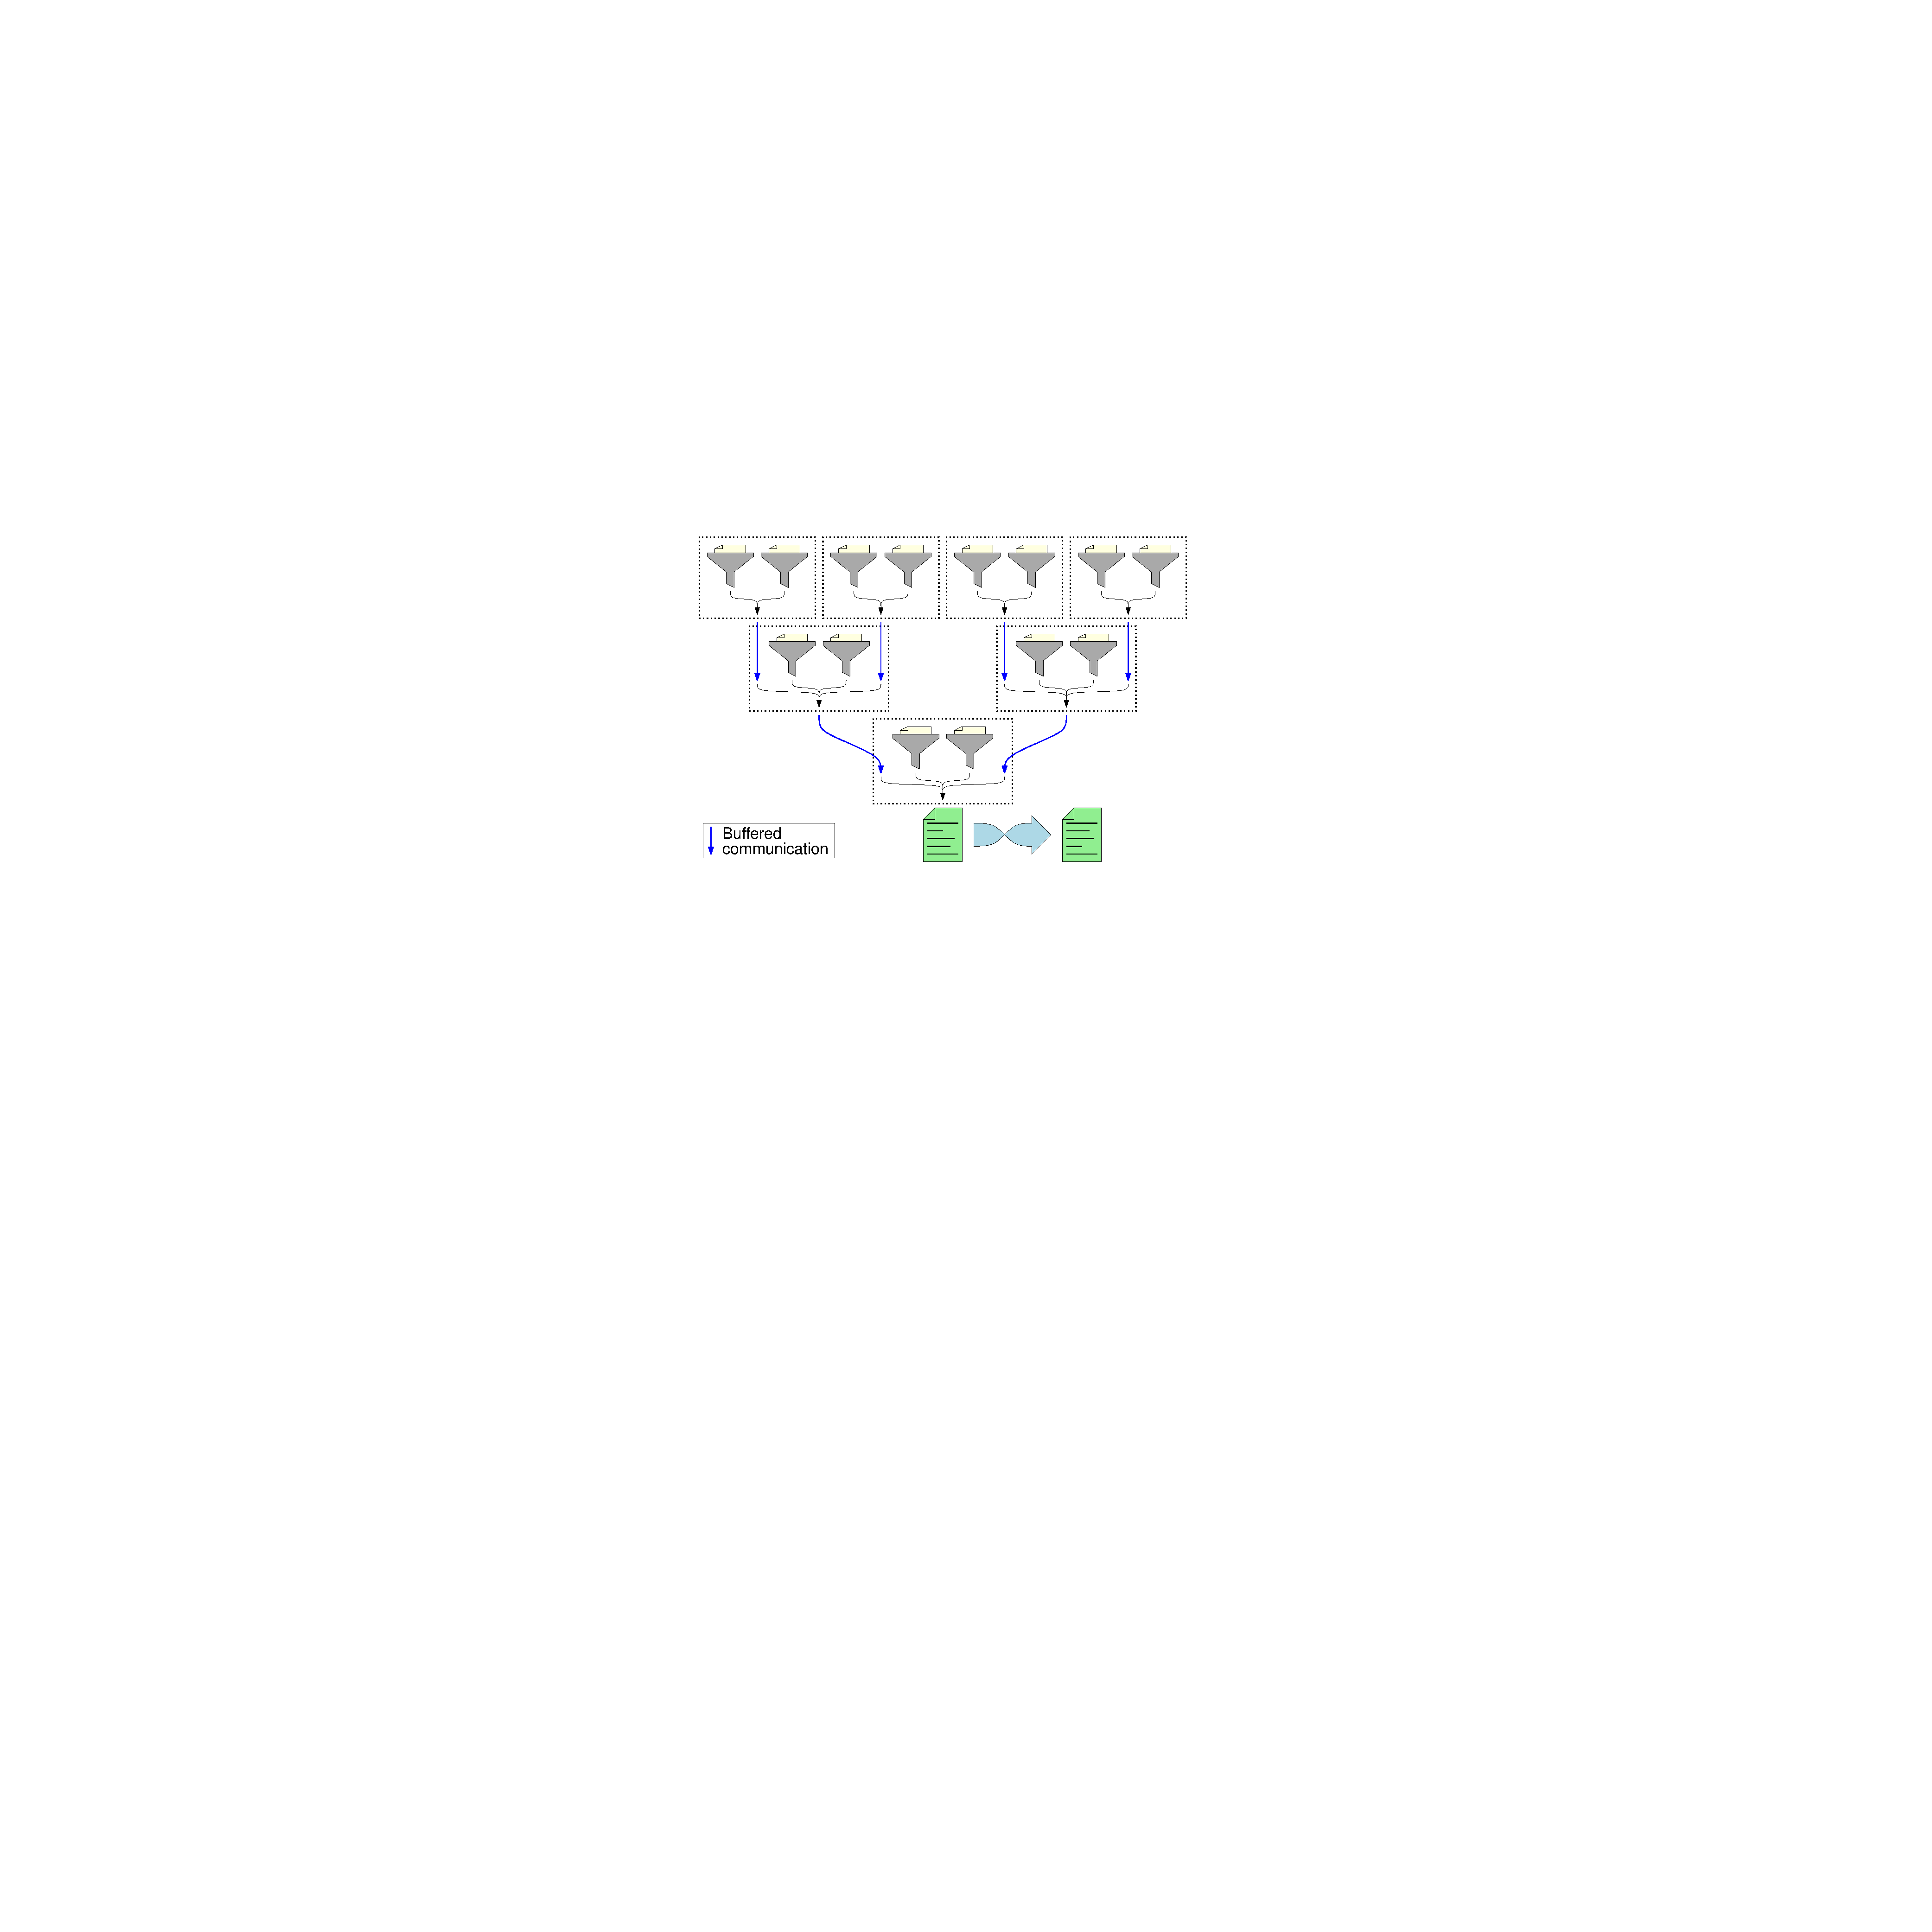
\includegraphics[width=\textwidth]{figures/l13/merging.pdf}
	\end{minipage}%
\end{frame}

\begin{frame}{Distributed Proof Production: Discussion}
	
	\textbf{Results:} \hfill\unimp{(Latest setup, JAR'24 submission)}
	\begin{itemize}
		\item Mean speedup of proof-emitting solver @ 1520 cores over sequential solver (solving times only): \highl{17.5}
		\begin{itemize}
			\item Mean speedup of best \textsc{MallobSat} @ 1520 cores over sequential solver: \highl{26.9}
		\end{itemize}
		\item On average, \highl{assembling and checking} a proof takes \highl{$\approx 3\times$ solving time}
		\begin{itemize}
			\item Mean overhead of DRAT proof checking over sequential solving: $\approx 1\times$
		\end{itemize}
		\item Pruning irrelevant clause additions \highl{reduces proof size by $\approx$ 30--40$\times$}
		\item LRAT proof size: median 3.1\,GB, mean 11.6\,GB, \highlo{maximum 233.9\,GB}
	\end{itemize}
	
	\vspace*{2mm}
	\textbf{Bottleneck:} \pause \highlo{Assembly and validation of a monolithic proof}
	\begin{itemize}
		\item Proof creation throttled by \highlo{I/O bandwidth at final process}
		\item Checking can \highlo{take very long}
		\item The assembled proof's ``corridor'' of active clauses may \highlo{no longer fit into RAM}
	\end{itemize}

	\vspace*{2mm}	
	\textbf{Can we do better?}
\end{frame}

\begin{frame}{Hermione's Answer to More Scalable Trusted Solving}
	
	\vspace*{4mm}
	\centering
	
\includegraphics[width=10cm]{figures/l13/pipes.jpg}\\
	\unimp{\footnotesize {https://i.pinimg.com/originals/1b/3d/b6/1b3db639721eeafb188a3cc3060ff58b.jpg}}
\end{frame}

\begin{frame}{Beyond Monolithic Proof Files}
	Marijn Heule: Since LRUP checking is so efficient, we can feasibly do it \highl{in realtime}!
	\begin{itemize}
		\item Solver streams proof output into a \highl{pipe} (UNIX special file)
		\item Checker reads proof from pipe and checks it \highl{on-the-fly}\\
		-- \highl{checking is done as soon as solving is done!}
		\item \highl{Almost no slowdown} when running solver and checker on \highl{two hardware threads of the same core}
		\item \highl{No disk I/O} required, \highl{same program code as with normal files} (execute \texttt{mkfifo} beforehand)
		\item \highlo{Does not yield a persistent artifact} to validate by independent parties
	\end{itemize}

	\vspace*{3mm}
	\begin{center}
		
\includegraphics[width=8cm]{figures/l13/pipe-setup.pdf}
	\end{center}
\end{frame}

\begin{frame}{Clause-Sharing Solving with on-the-fly Checking\ \ \cite{schreiber2024trusted}}
	\centering
	\vspace*{3mm}
	\hspace*{-6mm}\begin{minipage}[c][8cm][t]{0.5\textwidth}
		\begin{itemize}
			\item One checker per solver thread
			\item Incoming shared clauses are forwarded\\
			to the checker \highlo{without (LRUP) checking}
			\only<2>{\item How do we account for \highlo{incorrect shared clauses}?}%
			\item<3-> Checkers \highl{sign} each successfully checked clause $c$ with \highl{128-bit signature} based on
			\highl{shared secret $K$}:\\[1mm]
			$\mathcal{S}_K(c) = H_K(id(c)\ ||\ c\ ||\ \mathcal{S}_K(F))$
			\item<3->[] $H_K$: \highl{Message Authentication Code} (MAC), specifically \textbf{SipHash}
			\item<4-> Incoming clause $c$ is forwarded to checker\\
			\highl{together with $\mathcal{S}_K(c)$}\\
			$\Rightarrow$ Checker can validate that \highl{another}\\
			\phantom{$\Rightarrow$} \highl{checker has signed the clause}!
			%\item<4-> Stable run-time-overhead \highl{$\leq 42\%$}\\over normal solving ($\leq$ 2560 cores)\\
			%\mbox{\small --- Explicit proof production + checking: \highlo{$>600\%$}}
		\end{itemize}
	\end{minipage}
	\ \ \ 
	\begin{minipage}[c][8cm][t]{0.5\textwidth}
		\centering
		\vspace*{0.5cm}
		\ \ 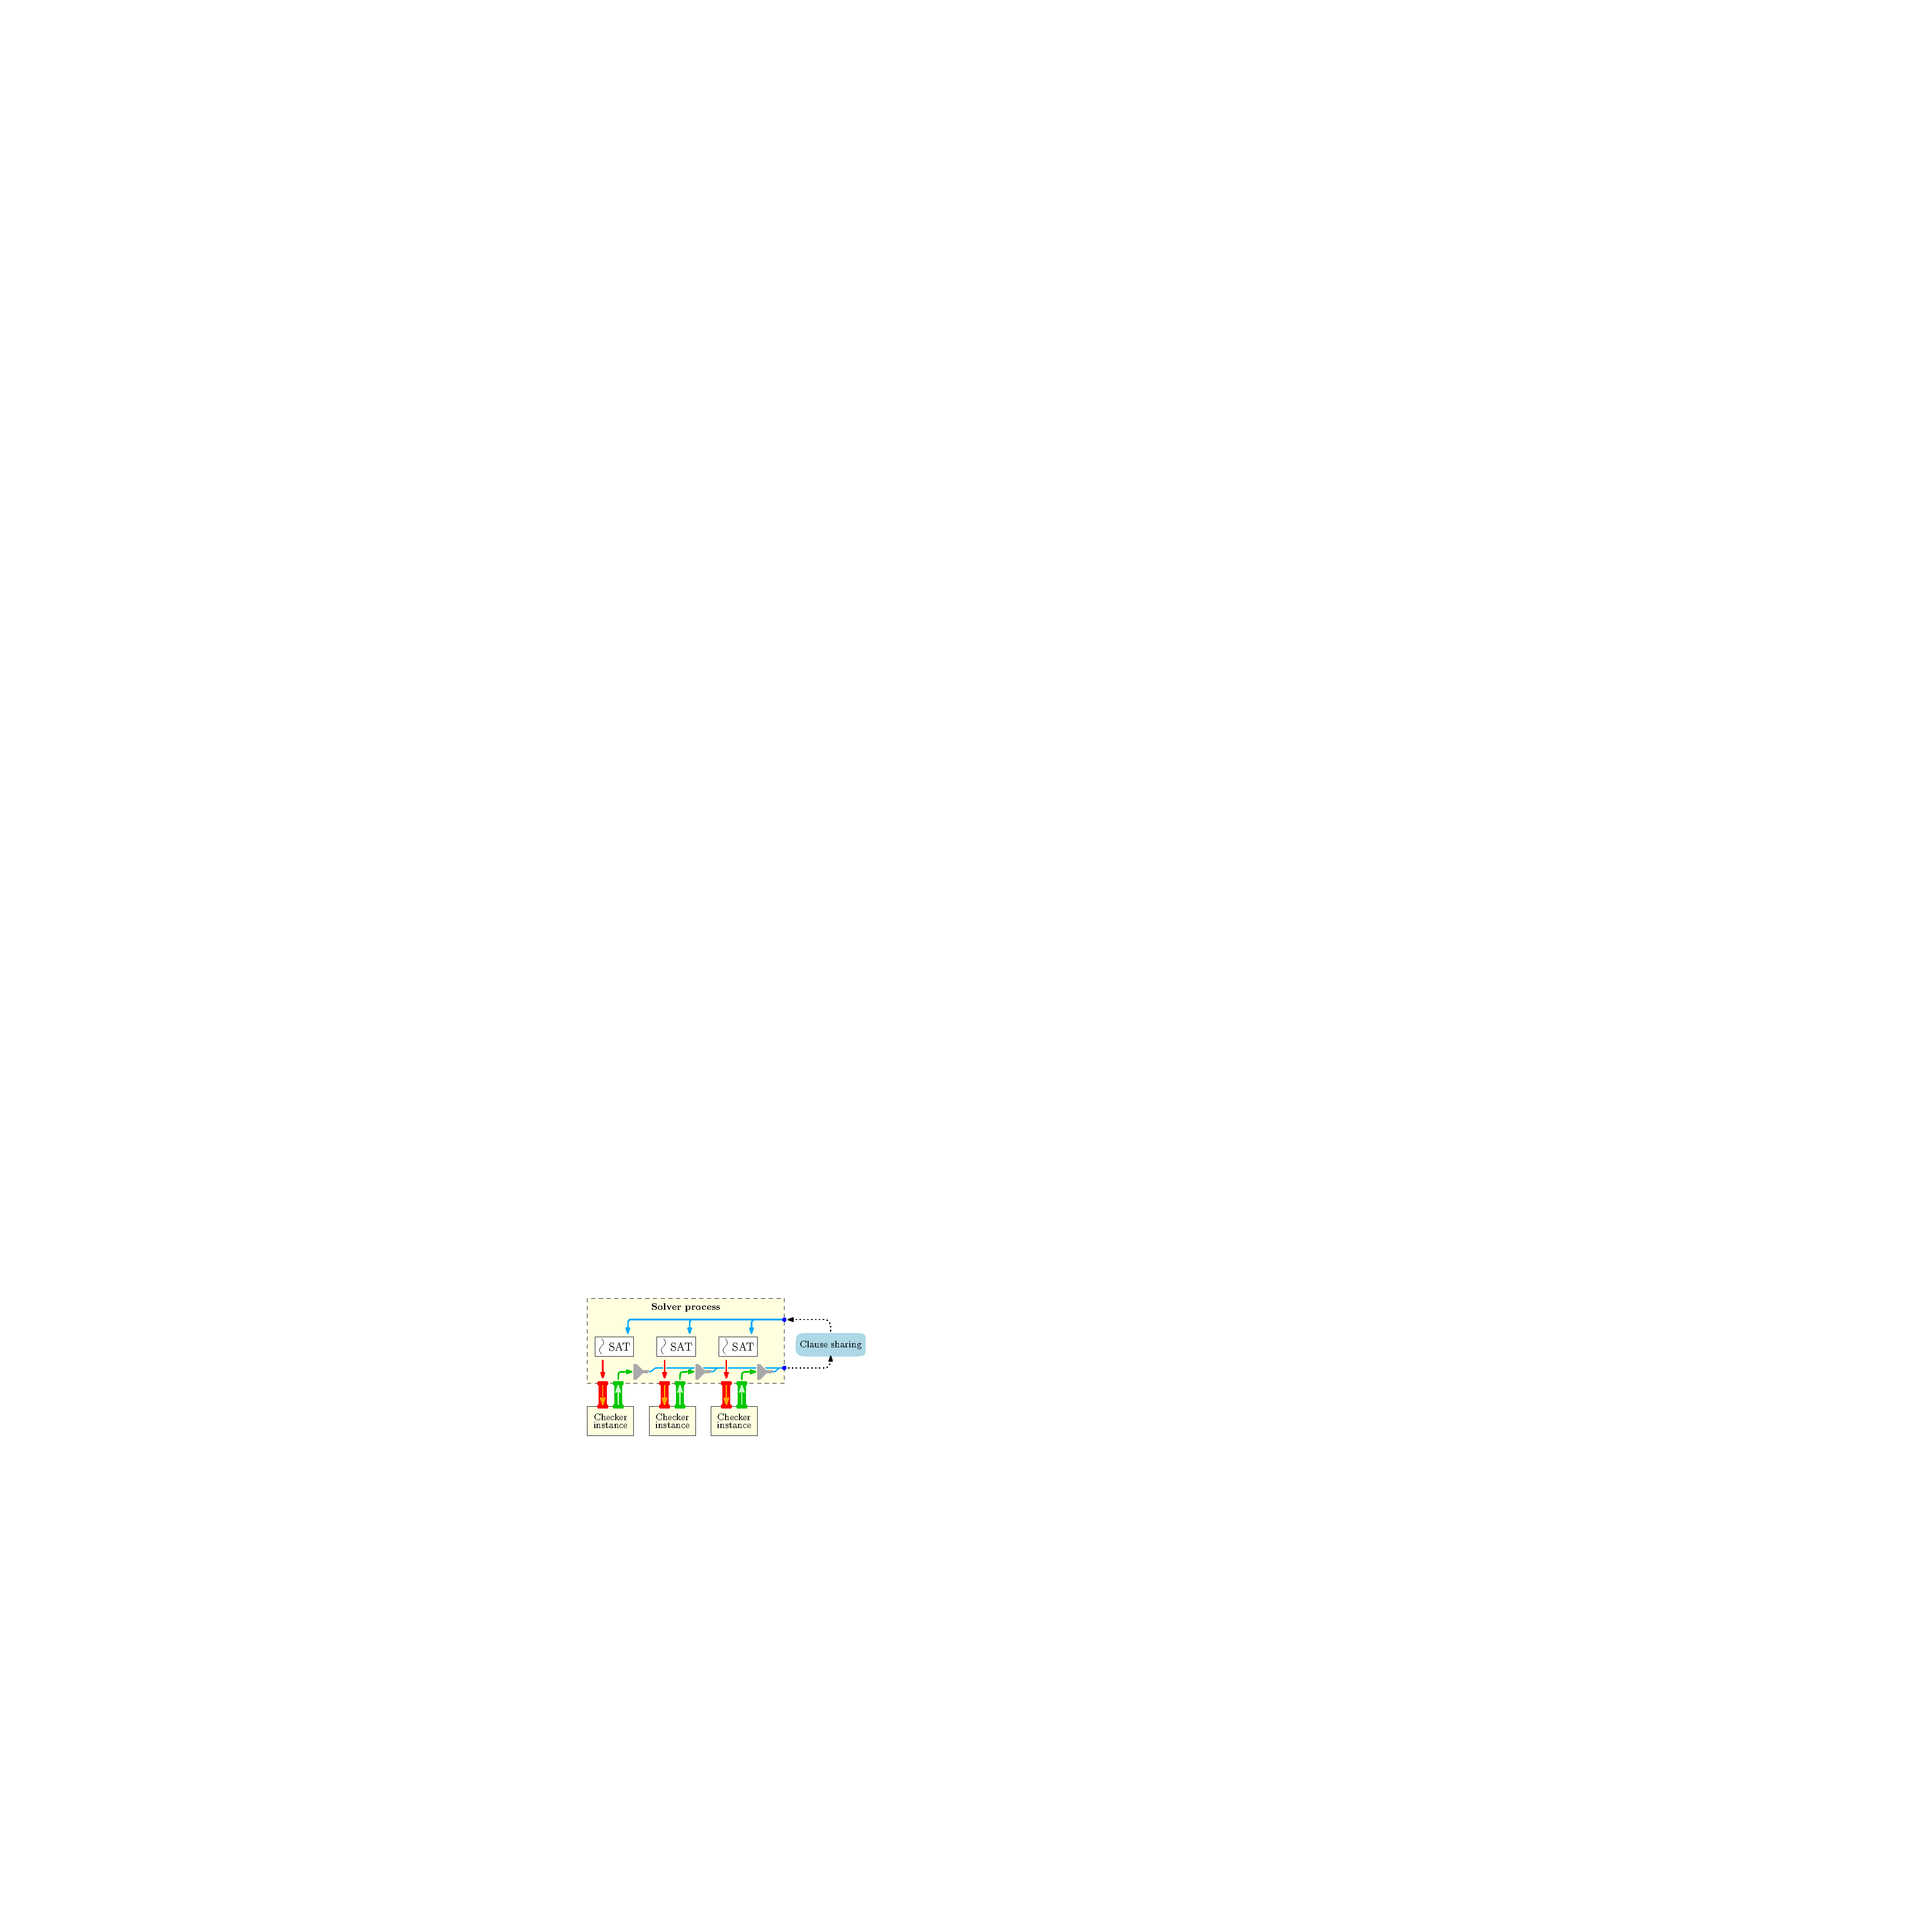
\includegraphics[width=\textwidth]{figures/l13/trusted-distributed-solving.pdf}\\
		
		\vspace*{0.5cm}
		\hfill\url{github.com/domschrei/impcheck}
	\end{minipage}%
\end{frame}

\begin{frame}{Clause-Sharing Solving + Checking: Scalability\ \ \cite{schreiber2024trusted}}
	
	\vspace*{-2mm}
	\begin{minipage}{0.315\textwidth}
		\centering
		On-the-fly checking\\[2mm]
		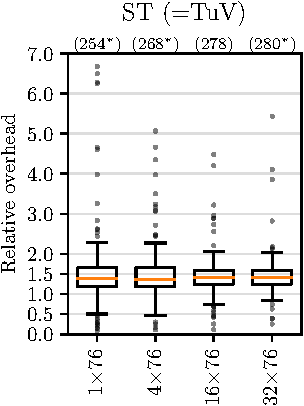
\includegraphics[scale=0.8]{figures/l13/boxplot-otfc.pdf}%	
	\end{minipage}\ \ 
	\begin{minipage}{0.67\textwidth}
		\centering
		Monolithic proofs\\[2mm]
		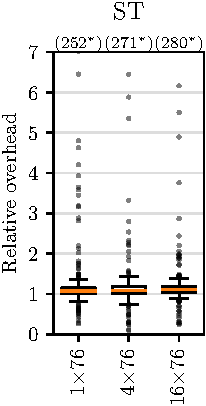
\includegraphics[scale=0.8]{figures/l13/boxplot-proof-qtimes.pdf}%
		\hspace*{2mm}%
		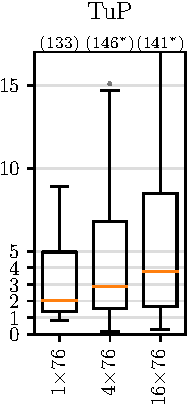
\includegraphics[scale=0.8]{figures/l13/boxplot-proof-qtup.pdf}%
		\hspace*{2mm}%
		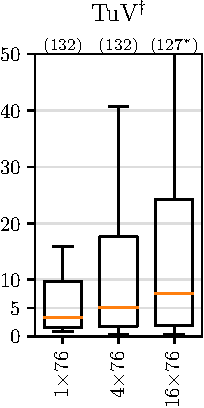
\includegraphics[scale=0.8]{figures/l13/boxplot-proof-qtuv.pdf}%
	\end{minipage}%

	\vspace*{0.5mm}
	\begin{center}
		\unimp{
			\footnotesize Overhead relative to proof-free solving time\ \ $\cdot$\ \ ST: Solving time\ \ $\cdot$\ \ TuP: Time until Proof present\ \ $\cdot$\ \ TuV: Time until Validation done\\[-1mm]
			76-core nodes\ \ $\cdot$\ \ $^\dagger$Data extrapolated\ \ $\cdot$\ \ $^*$some data outside of displayed domain
		}
	\end{center}
\end{frame}

\begin{frame}{Wrap-Up}
	\begin{itemize}
		\item \textbf{Proofs:} \highl{Powerful and practical technology} to ensure that a solver's result is correct
		\item \textbf{Proof formats:} Trade-off between \highl{expressivity}, \highl{checking efficiency}, and \highlo{solver development effort}
		\pause
		\item Highly efficient \highl{on-the-fly checking} is possible if \highlo{persistent proof artifact is expendable}
		\begin{itemize}
			\item \highl{Substantially more scalable} than explicit proof production in distributed solving
			\item Unclear if / how well this works for \highlo{actual LRAT} (not LRUP) derivations\\
			-- especially for \highlo{clause-sharing solving}
		\end{itemize}
		\pause
		\item \textbf{Right now:} Rise of \highl{new proof formats} (PR, PB, \ldots) promising shorter proofs for some problems~\cite{balyo2023proceedings}\\
		-- DRAT / LRAT is technically \highl{just as powerful} but relies on \highlo{variable addition} for most powerful proofs
		\begin{itemize}
			\item \highlo{huge decision space}, difficult to find a short proof
			\item But: recent success in effective \highl{structured variable addition}~\cite{haberlandt2023effective}
		\end{itemize}
	\end{itemize}
\end{frame}

\begin{frame}{References}
	\renewcommand*{\bibfont}{\scriptsize}
	\setlength\bibitemsep{3pt}
	\vspace*{-3mm}
	\printbibliography
\end{frame}

\end{document}
